%%%%%%%%%%%%%%%%%%%%%%%%%%%%%%%%%%%%%%%%%%%%%%%%%%%%%%%%%%%%%%%%%%%%%%%%%%%%%%%%%%%%%%%%%%%%%%%%%
%%%%%  Beamer Sildes  %%%%%%%%%%%%%%%%%%%%%%%%%%%%%%%%%%%%%%%%%%%%%%%%%%%%%%%%%%%%%%%%%%%%%%%%%%%
%%%%%%%%%%%%%%%%%%%%%%%%%%%%%%%%%%%%%%%%%%%%%%%%%%%%%%%%%%%%%%%%%%%%%%%%%%%%%%%%%%%%%%%%%%%%%%%%%

% https://en.wikibooks.org/wiki/LaTeX/Presentations

% \documentclass{beamer}
\documentclass{beamer}
\mode<presentation> {
% \mode<handout> {

    %%%%%  Themes  %%%%%%%%%%%%%%
    %%%%%%%%%%%%%%%%%%%%%%%%%%%%%
    % \usetheme{AnnArbor}
    % \usetheme{Antibes}
    % \usetheme{Bergen}
    % \usetheme{Berkeley}
    % \usetheme{Berlin}
    % \usetheme{CambridgeUS}
    % \usetheme{Copenhagen}
    % \usetheme{Darmstadt}
    % \usetheme{Dresden}
    % \usetheme{Frankfurt}
    % \usetheme{Goettingen}
    % \usetheme{Hannover}
    % \usetheme{Ilmenau}
    % \usetheme{JuanLesPins}
    % \usetheme{Luebeck}
    % \usetheme{Madrid}
    % \usetheme{Malmoe}
    % \usetheme{Marburg}
    % \usetheme{Montpellier}
    % \usetheme{PaloAlto}
    % \usetheme{Pittsburgh}
    % \usetheme{Rochester}
    % \usetheme{Singapore}
    % \usetheme{Szeged}
    % \usetheme{Warsaw}
    % \usetheme{boxes}
    \usetheme{default}

    %%%%%  Color Themes  %%%%%%%%
    %%%%%%%%%%%%%%%%%%%%%%%%%%%%%
    % \usecolortheme{default}
    % \usecolortheme{albatross}
    % \usecolortheme{beaver}
    % \usecolortheme{beetle}
    % \usecolortheme{crane}
    % \usecolortheme{dolphin}
    % \usecolortheme{dove}
    % \usecolortheme{fly}
    % \usecolortheme{lily}
    % \usecolortheme{orchid}
    % \usecolortheme{rose}
    % \usecolortheme{seagull}
    % \usecolortheme{seahorse}
    % \usecolortheme{whale}
    % \usecolortheme{wolverine}

    %%%%%  Outer Themes  %%%%%%%%
    %%%%%%%%%%%%%%%%%%%%%%%%%%%%%
    % \useoutertheme{infolines}
    % \useoutertheme{miniframes}
    % \useoutertheme{shadow}
    % \useoutertheme{sidebar}
    % \useoutertheme{smoothbars}
    % \useoutertheme{smoothtree}
    % \useoutertheme{split}
    % \useoutertheme{tree}

    %%%%%  Inner Themes  %%%%%%%%
    %%%%%%%%%%%%%%%%%%%%%%%%%%%%%
    % \useinnertheme{rectangles}
    % \useinnertheme{circles}
    % \useinnertheme{inmargin}
    % \useinnertheme{rounded}
}

\usepackage{amsthm}
\usepackage{amsmath}
\usepackage{amssymb}
\usepackage{array}
\usepackage[fleqn]{mathtools}
\usepackage{caption}
\usepackage{wallpaper}
\usepackage{xcolor}
\definecolor{umblue}{HTML}{00274C}
\definecolor{ummaize}{HTML}{FFCB05}
\usepackage{colortbl}
\usepackage{graphicx} 
\usepackage{pgf}
\usepackage{tikz}
\usetikzlibrary{arrows,automata}
\usepackage{url}			       
\usepackage{hyperref}

% \setbeamercolor{alerted text}{fg=orange}
% \setbeamercolor{background canvas}{bg=white}
% \setbeamercolor{block body alerted}{bg=normal text.bg!90!black}
% \setbeamercolor{block body}{bg=normal text.bg!90!black}
% \setbeamercolor{block body example}{bg=normal text.bg!90!black}
% \setbeamercolor{block title alerted}{use={normal text,alerted text},fg=alerted text.fg!75!normal text.fg,bg=normal text.bg!75!black}
% \setbeamercolor{block title}{bg=blue}
% \setbeamercolor{block title example}{use={normal text,example text},fg=example text.fg!75!normal text.fg,bg=normal text.bg!75!black}
% \setbeamercolor{fine separation line}{}
% \setbeamercolor{frametitle}{fg=brown}
% \setbeamercolor{item projected}{fg=black}
% \setbeamercolor{normal text}{bg=black,fg=yellow}
% \setbeamercolor{palette sidebar primary}{use=normal text,fg=normal text.fg}
% \setbeamercolor{palette sidebar quaternary}{use=structure,fg=structure.fg}
% \setbeamercolor{palette sidebar secondary}{use=structure,fg=structure.fg}
% \setbeamercolor{palette sidebar tertiary}{use=normal text,fg=normal text.fg}
% \setbeamercolor{section in sidebar}{fg=brown}
% \setbeamercolor{section in sidebar shaded}{fg=grey}
% \setbeamercolor{separation line}{}
% \setbeamercolor{sidebar}{bg=red}
% \setbeamercolor{sidebar}{parent=palette primary}
\setbeamercolor{structure}{bg=ummaize, fg=umblue}
% \setbeamercolor{subsection in sidebar}{fg=brown}
% \setbeamercolor{subsection in sidebar shaded}{fg=grey}
% \setbeamercolor{title}{fg=brown}
% \setbeamercolor{titlelike}{fg=brown}

% \setbeamertemplate{page number in foot}[appendixframenumber]
\setbeamertemplate{footline}[frame number]
% \setbeamertemplate{blocks}[rounded][shadow=true]
% \setbeamertemplate{background canvas}[vertical shading][bottom=white,top=structure.fg!25]
% \setbeamertemplate{sidebar canvas left}[horizontal shading][left=white!40!black,right=black]

\setbeamerfont*{footline}{family=\sffamily, size=\large}
% \setbeamerfont{title}{family=\rmfamily\addfontfeatures{Scale=1.18, Numbers={Lining, Proportional}}}
\usefonttheme[onlymath]{serif}

\beamertemplatenavigationsymbolsempty

\hypersetup{pdfstartview={Fit}} % fits the presentation to the window when first displayed

\newcommand{\XB}{\color{black}}
\newcommand{\XBB}{\color{blue}}
\newcommand{\XV}{\color{violet}}
\newcommand{\XR}{\color{red}}
\newcommand{\XUMB}{\color{umblue}}
\newcommand{\XUMM}{\color{ummaize}}

\newcommand{\ds}{\displaystyle}

% Use pause in math enviornments
\makeatletter
\renewrobustcmd{\beamer@@pause}[1][]{
  \unless\ifmeasuring@
  \ifblank{#1}
    {\stepcounter{beamerpauses}}
    {\setcounter{beamerpauses}{#1}}
  \onslide<\value{beamerpauses}->\relax
  \fi
}
\makeatother

%%%%%%%%%%%%%%%%%%%%%%%%%%%%%%%%%%%%%%%%%%%%%%%%%%%%%%%%%%%%%%%%%%%%%%%%%%%%%%%%%%%%%%%%%%%%%%%%%
%%%%%  Title Page  %%%%%%%%%%%%%%%%%%%%%%%%%%%%%%%%%%%%%%%%%%%%%%%%%%%%%%%%%%%%%%%%%%%%%%%%%%%%%%
%%%%%%%%%%%%%%%%%%%%%%%%%%%%%%%%%%%%%%%%%%%%%%%%%%%%%%%%%%%%%%%%%%%%%%%%%%%%%%%%%%%%%%%%%%%%%%%%%

\title[Factors Affecting Cloud ERP Adoption Decisions in Organizations]{Factors Affecting Cloud ERP Adoption Decisions in Organizations}
\author{\XV\textit{\large{\href{https://github.com/casonk}{Cason Konzer}}}\XB}
\institute[UM FLINT]{\normalsize{\textit{casonk@umich.edu}}}
\titlegraphic{
\includegraphics[scale = 0.5]{C:/Users/cason/OneDrive - Umich/Computer_Science/Classes/Spring_2023/CIS_562_Enterprise_Architecture/Week4/University_of_Michigan_Flint.png}}
\date[]{\today} 

\begin{document}

\begin{frame}
    \titlepage
\end{frame}


%%%%%%%%%%%%%%%%%%%%%%%%%%%%%%%%%%%%%%%%%%%%%%%%%%%%%%%%%%%%%%%%%%%%%%%%%%%%%%%%%%%%%%%%%%%%%%%%%
%%%%%  Begin Slides  %%%%%%%%%%%%%%%%%%%%%%%%%%%%%%%%%%%%%%%%%%%%%%%%%%%%%%%%%%%%%%%%%%%%%%%%%%%%
%%%%%%%%%%%%%%%%%%%%%%%%%%%%%%%%%%%%%%%%%%%%%%%%%%%%%%%%%%%%%%%%%%%%%%%%%%%%%%%%%%%%%%%%%%%%%%%%%

%%%%%  Paper Background  %%%%%%%%%%%%%%%%%%%%%%%%%%%%%%%%%%%%%%%%%%%%%%%%%%%%%%%%%%%%%%%%%%%%%%%%

\section{Paper Background}

\begin{frame}

    \frametitle{Paper Background}

    For this presentation will will study ``Factors Affecting Cloud ERP Adoption Decisions in Organizations,'' by Vilde Christiansen, Moutaz Haddara and Marius Langseth [1]. \pause

    \vspace{5mm}
    The paper was presented in CENTRIS, ProjMAN and HCist (2021) international conferences before being published in Procedia Computer Science at the beginning of 2022. \pause
    
    \vspace{2.5mm}
    \begin{itemize}
        \item[$\diamond$] CENTRIS - International Conference on ENTERprise Information Systems. \pause
        \item[$\diamond$] ProjMAN - International Conference on Project MANagement. \pause
        \item[$\diamond$] HCist - International Conference on Health and Social Care Information Systems and Technologies.
    \end{itemize}

\end{frame}

%%%%%  Introduction  %%%%%%%%%%%%%%%%%%%%%%%%%%%%%%%%%%%%%%%%%%%%%%%%%%%%%%%%%%%%%%%%%%%%%%%%%%%%

\section{Introduction}

\begin{frame}

    \frametitle{Introduction}

    The paper as presented is a literature review, or meta-study, which aims to bridge findings across multiple studies and form a general consensus. \pause

    \vspace{3.33mm}
    Focus is given on SMEs (small and medium-size enterprises), along side LEs (large enterprises), identifying similarities and differences between them. \pause

    \vspace{3.33mm}
    Industry trends are showing a move from on-premise to cloud ERP (enterprise resource planning) systems, with a 2020 report by Panorama Consulting Group finding a 62.7\% adoption rate. \pause
    
    \vspace{3.33mm}
    More over, the implementations are most often seen as SaaS (software as a service) solutions, about 90\%, minimizing the time to go-live.

\end{frame}

\begin{frame}

    \frametitle{Business Sizes}

    \centering
    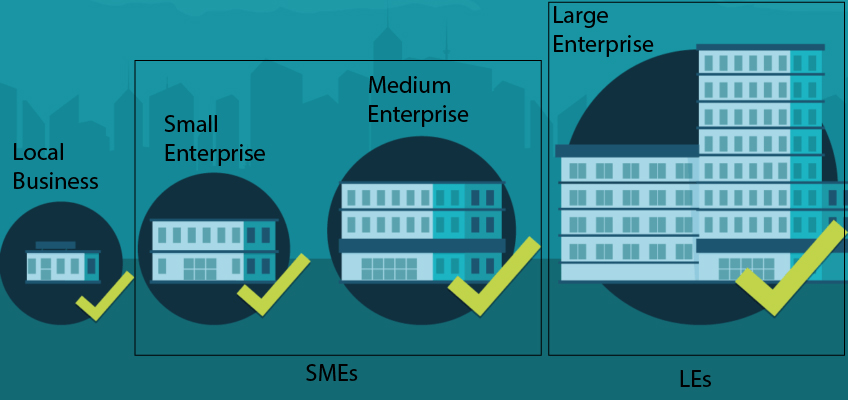
\includegraphics[scale = 0.33]{C:/Users/cason/OneDrive - Umich/Computer_Science/Classes/Spring_2023/CIS_562_Enterprise_Architecture/Week4/enterprise_sizes.jpg}

    \footnotesize {\url{https://desmotechsolutions.com/desmo-tech-solutions-small-medium-business/}}

\end{frame}

\begin{frame}

    \frametitle{Cloud Offerings}

    \centering
    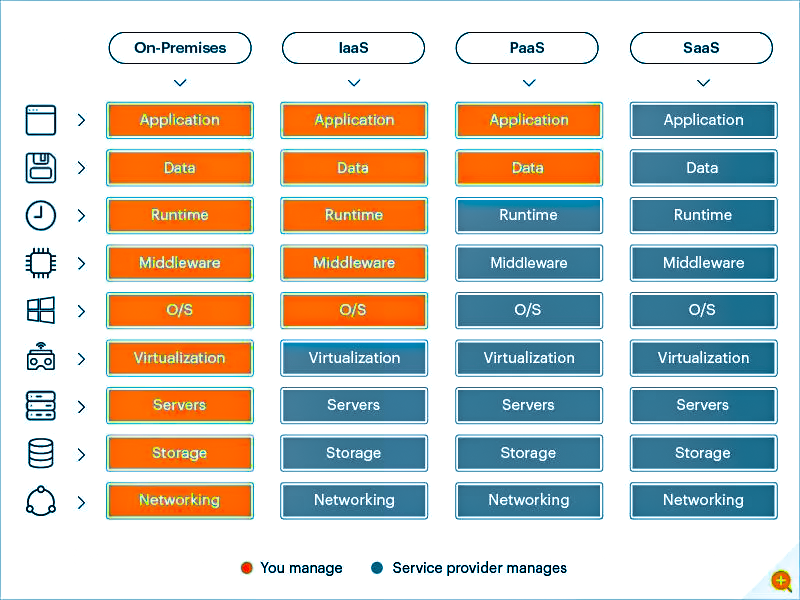
\includegraphics[scale = 0.33]{C:/Users/cason/OneDrive - Umich/Computer_Science/Classes/Spring_2023/CIS_562_Enterprise_Architecture/Week4/Onsite-Iaas-Paas-Saas.png}

    \footnotesize {\url{https://www.eginnovations.com/blog/saas-vs-paas-vs-iaas-examples-differences-how-to-choose/}}

\end{frame}

%%%%%  Research Question  %%%%%%%%%%%%%%%%%%%%%%%%%%%%%%%%%%%%%%%%%%%%%%%%%%%%%%%%%%%%%%%%%%%%%%

\section{Research Question}

\begin{frame}

    \frametitle{Research Question}

    The primary research question addressed is:
    \begin{itemize}
        \item[$\ast$] ``What are the main factors affecting the decision to adopt cloud ERP at the organizational level in the extant literature?'' \pause
    \end{itemize}

    \vspace{5mm}
    Generally speaking the authors wonder why organizations are making the move to the cloud, identifying the pros and cons of such a decision. 

\end{frame}

%%%%%  Methodology  %%%%%%%%%%%%%%%%%%%%%%%%%%%%%%%%%%%%%%%%%%%%%%%%%%%%%%%%%%%%%%%%%%%%%%%%%%%%

\section{Methodology}

\begin{frame}

    \frametitle{Methodology}

    As this paper is a literature review, the methodology borrows a well document method from [2]. \pause

    \vspace{5mm}
    The steps can be summarized as follows:
    \begin{enumerate}
        \item Formulation of the Research Question. \pause
        \item Localization of the Articles. \pause
        \item Selection and Evaluation of the Studies. \pause
        \item Analysis and Synthesis. \pause
        \item Development of Report with Findings. 
    \end{enumerate}

\end{frame}

\begin{frame}

    \frametitle{Localization of the Articles}

    Articles were found through a pairing of search keywords utilizing Oria's database. \pause

    \vspace{5mm}
    The search is summarized by an \emph{and} condition across the following clauses.
    \begin{itemize}
        \item[$\diamond$] Cloud \emph{or} Cloud-Based \emph{or} Software as a Service. \pause
        \item[$\diamond$] ERP \emph{or} Enterprise Resource Planning. \pause
        \item[$\diamond$] DOI \emph{or} TBP.
    \end{itemize} \pause

    \vspace{5mm}
    \footnotesize 
    Note: \\
    DOI - Diffusion of Innovation. \\
    TBP - undefined.


\end{frame}

\begin{frame}

    \frametitle{Selection and Evaluation of the Studies}

    Utilizing the search framework, a total of 40 articles were located. \pause

    \vspace{5mm}
    The selection process imposed the following requirements:
    \begin{itemize}
        \item[$\diamond$] Inclusion of Cloud ERP Adoption Decisions. \pause
        \item[$\diamond$] Exclusion of Strictly Integration Phase Based Literature. \pause
        \item[$\diamond$] Disclosure of Organization Size(s).
    \end{itemize} \pause

    \vspace{5mm}
    In total 9 of the 40 articles were included, spanning 5 unique hosting databases.

\end{frame}

\begin{frame}

    \frametitle{Summary of Articles}

    \centering
    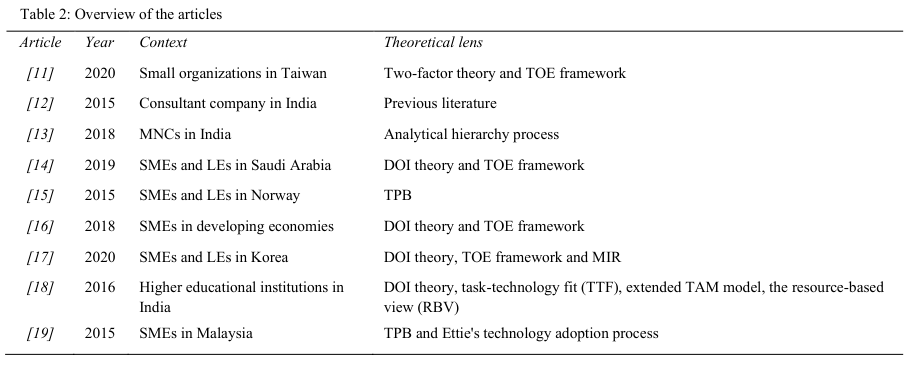
\includegraphics[scale = 0.44]{C:/Users/cason/OneDrive - Umich/Computer_Science/Classes/Spring_2023/CIS_562_Enterprise_Architecture/Week4/summary_of_articles.PNG}

    \footnotesize {[1, pg. 257]}

\end{frame}

%%%%%  Analysis  %%%%%%%%%%%%%%%%%%%%%%%%%%%%%%%%%%%%%%%%%%%%%%%%%%%%%%%%%%%%%%%%%%%%%%%%%%%%%%%

\section{Analysis}

\begin{frame}

    \frametitle{Analysis}

    As shown in `Summary of Articles' (Table 2: Overview of the articles) the authors managed to review literature across 6 years, including various contexts and theoretical perspectives. \pause

    \vspace{5mm}
    Similar to the findings in [3], the context of the organizations played a key role in the factors of concern. \pause

    \vspace{5mm}
    As a result we will provide a meta-summary of the most influential factors in cloud-ERP adoption across various contextual settings, as presented in the paper's discussion. 

\end{frame}

\begin{frame}

    \frametitle{Meta-Summary of Cloud-ERP Adoption Factors}

    \centering
    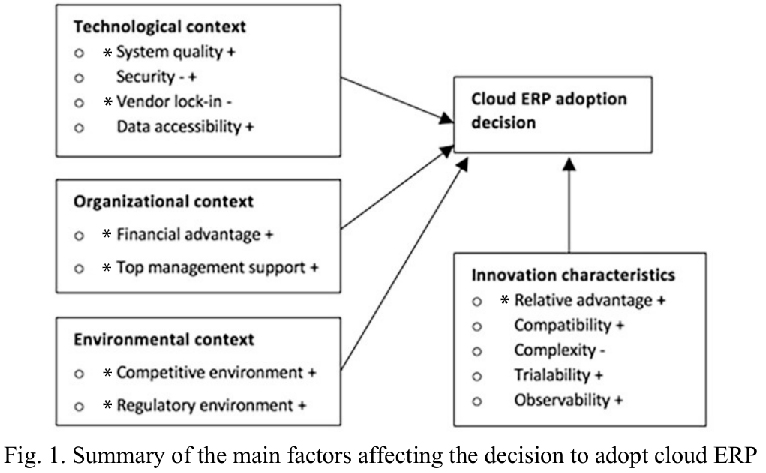
\includegraphics[scale = 0.33]{C:/Users/cason/OneDrive - Umich/Computer_Science/Classes/Spring_2023/CIS_562_Enterprise_Architecture/Week4/adoption_factors.jpg}

    \footnotesize {[1, pg. 261]}

\end{frame}

%%%%%  Conclusion  %%%%%%%%%%%%%%%%%%%%%%%%%%%%%%%%%%%%%%%%%%%%%%%%%%%%%%%%%%%%%%%%%%%%%%%%%%%%%

\section{Conclusion}

\begin{frame}

    \frametitle{Conclusion}

    Across the paper system quality, vendor lock-in, financial advantage, top management support, competitive environment, regulatory environment, and relative advantage were the most relevant factors in cloud-ERP adoption for SMEs and LEs. \pause

    \vspace{5mm}
    Of these, system quality and financial advantage showed the largest differences between SMEs and LEs. \pause

    \vspace{5mm}
    A common lack of differentiation between small, medium and large enterprises was noticed throughout the literature. \pause
    
    \vspace{5mm}
    As a result future research suggests finer grain study with respect to the distinguishing factor of business size. 

\end{frame}

%%%%%  Opinion  %%%%%%%%%%%%%%%%%%%%%%%%%%%%%%%%%%%%%%%%%%%%%%%%%%%%%%%%%%%%%%%%%%%%%%%%%%%%%%%%

\section{Opinion}

\begin{frame}

    \frametitle{Opinion}

    The authors of this paper were both clear and concise. \pause

    \vspace{5mm}
    Their methodology adopted an established procedure and their factor categorization utilized frequented theoretical frameworks. \pause

    \vspace{5mm}
    In analysis fine grained details were provided highlighting differences seen based on the economic situation, locality, and business size and viewed in the summarized papers. \pause

    \vspace{5mm}
    The meta-summary provided a clear overview of the cloud-ERP adoption landscape and conclusion provided suggestions for future research. 

\end{frame}

%%%%%  References   %%%%%%%%%%%%%%%%%%%%%%%%%%%%%%%%%%%%%%%%%%%%%%%%%%%%%%%%%%%%%%%%%%%%%%%%%%%%

\begin{frame}
    \frametitle{References}

    [1] V. Christiansen, M. Haddara, and M. Langseth, “Factors Affecting Cloud ERP Adoption Decisions in  Organizations,” Procedia Computer Science, vol. 196, pp. 255–262, 2022. [Online]. Available: \url{https://www.sciencedirect.com/science/article/pii/S1877050921022353}

    \vspace{2.5mm}
    [2] Denyer, David and David Tranfield, “Producing a Systematic Review”, The Sage Handbook of Organizational Research Methods, 2009.

    \vspace{2.5mm}
    [3] J. V. Gavidia, I. A. Junglas, and C.-H. Chou, “An integrated model of erp success: the critical role of task-context alignment,” Enterprise Information Systems, vol. 17, no. 1, p. 1931460, 2023.
    % \bibliography{konzer_cason_CIS_562_midterm_presentation.bib}
    % \bibliographystyle{ieeetran}

\end{frame}

\end{document} 

